\documentclass[12pt]{article}
\usepackage{graphicx}
\usepackage{listings}
\usepackage[tmargin=1in,bmargin=1in,lmargin=1.25in,rmargin=1.25in]{geometry}
\usepackage[nottoc,numbib]{tocbibind}

\begin{document}
%----------------------------------------------------------------------------------------
\begin{titlepage}

\newcommand{\HRule}{\rule{\linewidth}{0.5mm}}

\center
 
\textsc{\LARGE Lund University}\\[1.5cm]
\textsc{\Large Faculty of Engineering}\\[0.5cm]
\textsc{\large Applied Artificial Intelligence}\\[0.5cm]

\HRule \\[0.4cm]
{ \Large \bfseries Assignment 1: The Reversi Game}\\[0.1cm]
\HRule \\[1.5cm]
 
\Large \emph{Author:}\\
Nicolas \textsc{Burguer}\\
Juan Gabriel \textsc{Mart\'{i}nez Peris}\\[3cm]


\includegraphics[scale=0.35]{logo.png}\\[1cm] % Include a department/university logo - this will require the graphicx package 

\vfill % Fill the rest of the page with whitespace

\end{titlepage}
%----------------------------------------------------------------------------------------
\tableofcontents
\newpage
\section{Introduction}
%%--Background--%%
Artificial Intelligence(AI) and the videogame industry have a close relationship. Programmers working in that industry try to find better algorithms capable of winning a human player. There are different techniques depending on the type of game, but usually behind all of them there is a search algorithm that allows the computer to take the best decision depending on the state of the game.\\
\\ 
%%--The Problem--%%
The aim of this report is to explain our implementation of the \emph{Reversi/Othello} game, a popular board game created in 1883. It is played on an 8x8 board by two players, one of them will use dark disks and the other light ones. For the \emph{Othello} variant, the game starts with four discs placed in a square in the middle of the grid,  two facing light side up, two pieces with the dark side up, with same-colored disks on a diagonal with each other. In order to win the game, you must have more discs of your color than your opponent. You can achieve this by turning over any discs from your opponent that are in a straight line and bounded by the disk you have just placed and another of your disks.\\
\\
%%--The outline--%%
In the following sections are described our design with a UML diagram and the different Java classes with their methods. Furthermore, you will have explained how to execute our program and where to find it.  The last section has the conclusions that we have reached after finishing the assignment. 
\section{Design}
In this section we have described the design of our implementation. First, you will find the UML diagram with the classes and methods that we thought were necessary for the assignment. Then, we have highlighted some parts of the code in each class that are relevant in order to understand how the program works.
\newpage  
\subsection{UML Diagram}
\begin{figure}[h!]
	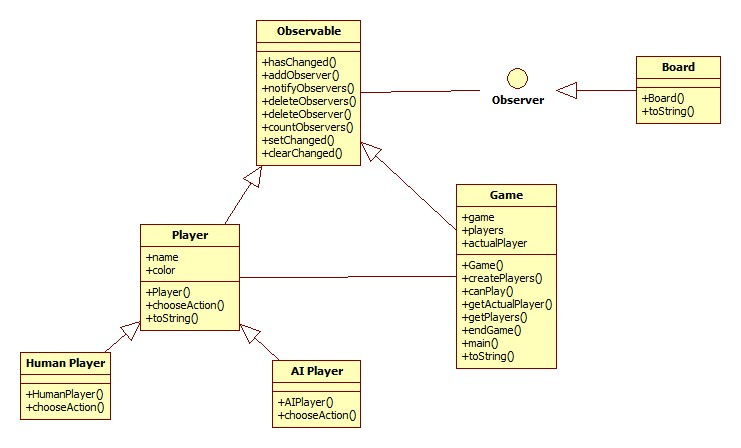
\includegraphics[scale=0.60]{Main.jpg}
	\caption{Othello's UML Diagram}
\end{figure}

\noindent Figure 1 shows the UML diagram of our \emph{Othello}'s implementation. As shown, we have 5 classes: Board, Game, Player, HumanPlayer and ArtificialIntelligence. We will describe the purpose of each of them briefly as we will highlight relevant pieces of code in the following subsections:
\begin{itemize}
	\item Board:
	\item Game:
	\item Player:
	\item HumanPlayer:
	\item ArtificialIntelligence:
\end{itemize} 
\subsection{Board.java}
\begin{lstlisting}[language=Java]
	System.out.println("Hello World");
\end{lstlisting}
\subsection{Player.java}
\subsection{ArtificialIntelligence.java}
\subsection{HumanPlayer.java}
\subsection{Game.java}
\section{Execution}
\section{Conclusion}
\begin{thebibliography}{9}
	\bibitem{WikiReversi}Reversi - Wikipedia entry: http://en.wikipedia.org/wiki/Reversi
	\bibitem{Russel} Russel, Stuart; Norvig, Peter, \emph{Artificial Intelligence, A Modern Approach}, Pearson Education, 3rd Edition.
\end{thebibliography}
\end{document}